\chapter{Discussion}

\section{Results}

Harmonic Onset Detector had the highest score on average of two datasets. On GuitarSet, the algorithm performed poorly in two cases. First, if the duration between two onsets is less than the size of the smoothing window (148 ms), there is a chance of failure to detect both onsets, depending on the difference of energies introduced by those onsets and how close they are. Onsets closer than 148 ms are not common and they are not existent in MusicCritic dataset. Second, the algorithm does not detect dead notes\footnote{Dead notes are intentionally created percussive, non-pitched sounds.}. Dead notes are common on chord recordings of the GuitarSet and they are annotated as onsets. For this reason, the recall of the algorithm is low on chords (Table \ref{tab:threeGS}). On MusicCritic dataset, one limiting factor is the time accuracy. In chords, annotations are usually close to the middle of the strum, and the algorithm usually predicts the beginning of the strum as the onset. Due to strums generally being slow in this dataset, the predictions were not always inside the tolerance window. Scores of all three algorithms are increased continuously with the size of the tolerance window (Figure \ref{fig:wsize_mc}). Same effect was not observed in GuitarSet (Figure \ref{fig:wsize_gs}).  

MC-OnsetDetector algorithm applies two restrictions after the Superflux algorithm. It requires the RMS difference of two consecutive frames to be positive and spectral centroid to be smaller than a constant. These restrictions are found to be problematic and the reasons of low recall of the algorithm on GuitarSet. A glissando does not necessarily increase the energy, so can not be detected due to RMS difference restriction. Spectral centroid of the high frequency notes usually have larger spectral centroid than most of the noises, and the spectral centroid of a buzz noise can be even smaller than a low frequency note. These restrictions did not have the same detrimental effect on MusicCritic dataset. The first reason is, the RMS difference feature is useful against buzz noises (although buzz noises may increase the energy). Second, MusicCritic dataset does not contain many high frequency notes, which makes the spectral centroid a better feature to eliminate slide noises. In Figure \ref{fig:mc217}, the recording contains three distinct notes, F5 (698 Hz), G5 (783 Hz) and A5 (880 Hz). Due to the spectral centroid limitation, only the F5 notes are predicted correctly.  

CNNOnsetDetector obtained the highest recall and the lowest precision values on both datasets. It detects more onsets than other algorithms by a large margin, but it falsely predicts guitar noises as onsets too. Those false predictions are expected for two reasons. First, It is trained to detect various kinds of instruments. Noises in guitar recordings may have similar characteristics to onsets of other instruments (e.g. percussion instruments) in the training dataset of the neural network. Second, by tracking the information about the dataset in \cite{schluter2014improved} it can be assumed that the dataset which CNNOnsetDetector was trained does not contain any amateur guitar recordings. Therefore the neural network can not discriminate the guitar noises from guitar notes.

The algorithms are also evaluated on the guitar noises dataset. The dataset contains 36 buzz and 234 slide noises. The number of mistakes of the algorithms are; Harmonic Onset Detector 118 (29 buzz), MC-OnsetDetector 160 (5 buzz), CNNOnsetDetector 247 (29 buzz). These numbers do not represent the performance of algorithms in a realistic recording because (1) The noises of the dataset are intentionally exaggerated. (2) Some thresholds (e.g. for RMS, Spectral Flux) in algorithms depend on the existence of played notes in the audio (e.g. some slide noises are very quiet and eliminated by energy threshold). Harmonic Onset Detector performs quite poor on buzz noises for the following reasons: Buzz noises cause a decrease in frequency depending on the finger location (section \ref{buzzsection}) and the noises in the dataset are created by pressing the left side of the frets, which causes greater frequency decrease. Additionally, the player tried to keep the buzzing of the strings as long as possible. Since the algorithm seeks for new harmonic content for a long duration in a true onset, it fails on these extreme conditions of buzz noises. Such exaggerated buzz noises are only possible to find on performances of beginner players (e.g. when beginners try to play barre chords). The constant values of the algorithm can be adjusted to work better on beginner performances, which would make it worse on advanced performances. The automatic calculation of such constants could increase the overall performance of the algorithm.

Usage of the differences between the onsets decreased the MSE of the automatic rhythm assessment system (Table \ref{tab:allassessment}). MSE is higher with CNNOnsetDetector algorithm (Table \ref{tab:allassessment}), which can be explained with its poor performance on MusicCritic dataset (Table \ref{tab:threeMC}). Interestingly, ground truth onsets did not yield lower MSE than the onset predictions of Harmonic Onset Detector and MC-OnsetDetector, whose F-scores are 0.85 and 0.80. This result supports our argument in the onset processing method (see \ref{assessmethod}). The current onset detection evaluation can not distinguish between an algorithm that misses the tolerance window randomly and the one that misses consistently and we argued that each algorithm would be consistent even if they miss the tolerance window. The scores of Harmonic Onset Detector and MC-OnsetDetector are both increased to 0.95 when the tolerance window is increased from 50 ms to 100 ms (Figure \ref{fig:wsize_mc}), which showed that their predictions are mostly accurate but sometimes slightly out of the tolerance window. Their consistency can be seen in the example in Figure \ref{fig:hodmcod215}. Since the onset differences were similar for the ground truth onsets and both algorithms' onset predictions, the grade predictions were also similar. There are downsides of using only the onset differences. First, the average offset between notes and the metronome beats is lost (e.g. If all the notes are played late by same amount, the deviation of differences will be zero). Second, the differences between notes and metronome beats are needed for feedback to the students.


\section{Evaluation of Onset Detection}

In MIREX results\footnote{https://nema.lis.illinois.edu/nema\_out/mirex2018/results/aod/index.html}, the score of the CNNOnsetDetector on plucked strings category is reported as 0.90, which is significantly different than its scores in GuitarSet and MusicCritic dataset. For further examination, we evaluated the algorithm on MusicNet\footnote{MusicNet has a large amount of various classical music recordings. Nearly half of the recordings are solo piano (917 minutes), followed by string quartet (405 minutes)} \cite{thickstun}. F-score of CNNOnsetDetector is found to be 0.62 on MusicNet, which is again significantly lower than its reported scores on related categories (Complex: 0.82, Solo Sustained String: 0.77, Solo Winds: 0.78, Poly Pitched: 0.95). 

The difference between the scores of CNNOnsetDetector in our experiments and MIREX results raises concerns about the reliability of MIREX evaluations. The dataset used in MIREX evaluations (MIREX05 dataset\footnote{https://www.music-ir.org/mirex/wiki/2005:Audio\_Onset\_Detect}) contains only 14 minutes of recordings. It contains commercial recordings and excerpts from RWC database\footnote{https://staff.aist.go.jp/m.goto/RWC-MDB/}. This dataset may not be appropriate for accurate evaluations, thus fair comparisons of algorithms. There is a need of a new and larger test dataset for the onset detection task.

For the evaluations of onset detection algorithms in our work, the standard evaluation method was adopted at first. Then, we shifted the predicted onset values and changed the tolerance window sizes to understand the behaviour of the algorithms. Such plots were used for further clarification in some other studies too, e.g. \cite{holzapfel2009three}. This means that the standard evaluation method is not descriptive enough to make comparisons. When a framework for musical onset detection task is first introduced, it is assumed that a prediction should be classified as correct or false, and a prediction at time t is counted as correct if there exists a true onset within a time frame \([t - \tau, t + \tau]\) \cite{leveau2004}. The tolerance window (\(\tau\)) is later accepted as 50 ms \cite{bello2005tutorial}. According to this assumption, a prediction 50.1 ms away from a true onset is not different than the one 10 seconds away. Both of them are classified as false predictions, so making no prediction at all is considered to be better. For example, in Figure \ref{fig:hodmcod215}, if an algorithm correctly predicts 7 out of 16 chords and make no predictions for 9 remaining chords, it will achieve higher scores than the shown algorithms. This evaluation method does not explain well how an algorithm behaves, at least for our application. 

Onset detection is the first stage of many MIR applications and different applications naturally have different needs. An evaluation method that compares onset detection algorithms should provide useful information for all applications. For this purpose, metrics of the evaluation should fit the nature of the onset detection task. Classes, such as "true" and "false", implies the existence of distinctive qualities between things. There is no such quality that makes a prediction with 50 ms error true and but the one with 51 ms false, or all the predictions below 50 ms equally true and the ones above equally false. If we suggest a metric that depends on distances directly, instead of true-false classes, then we would need another threshold for matching predictions to ground truth onsets for the following reason: If we match the closest ground truth - predicted onset pairs without a threshold, the distance between a pair can be very large. For an algorithm that only uses, say, 100 ms around time instants to make predictions, a pair with a distance more than 100 ms does not make sense. In that case, the prediction should be classified as false, as it can not be associated with a ground truth onset. One option would be to set a threshold to define false predictions and use distance metrics to elaborate on true onsets. 


\begin{figure}
    \centering
    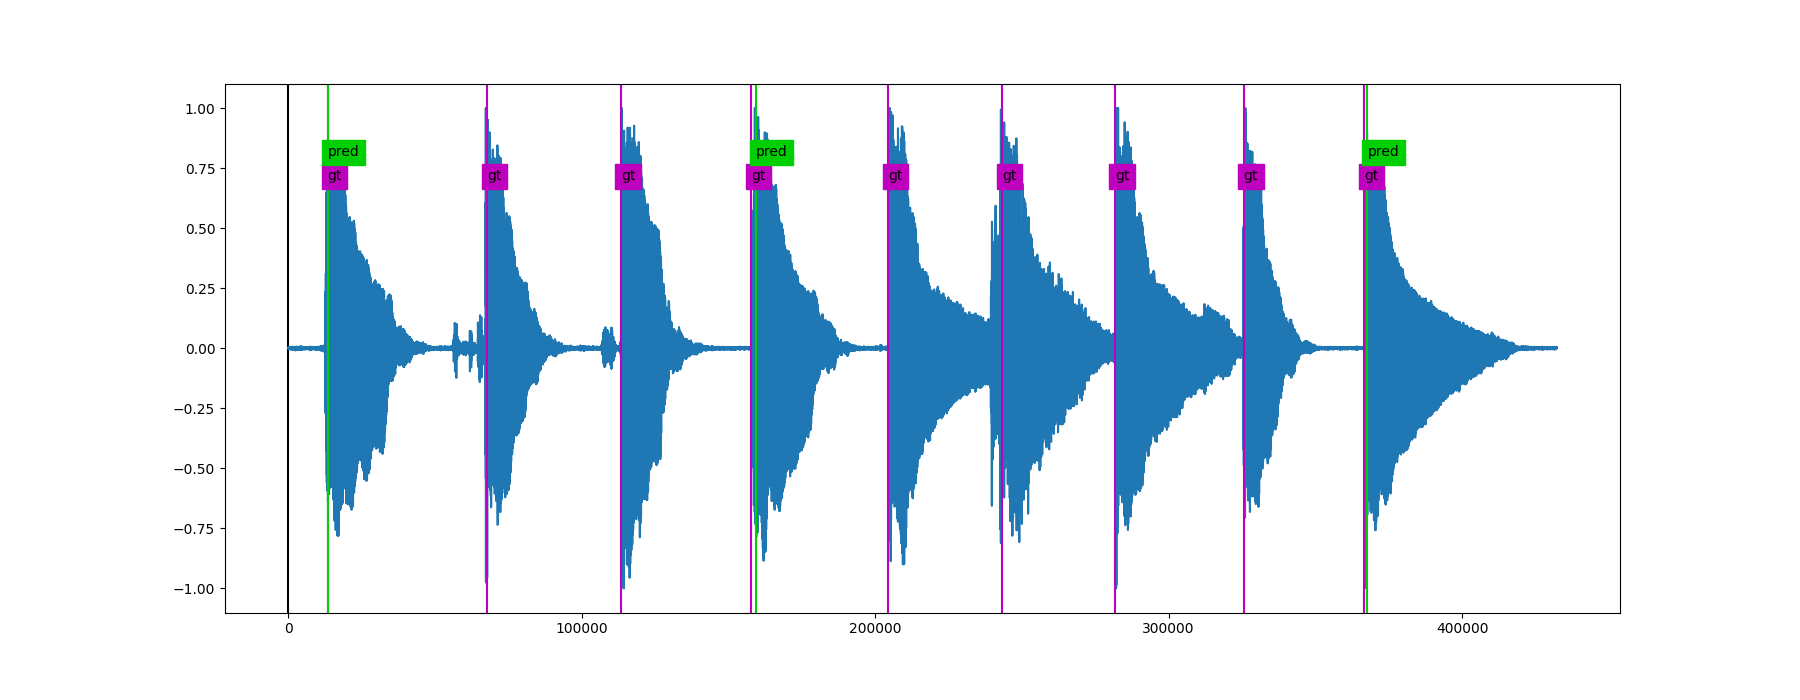
\includegraphics[width=\columnwidth]{discussion/MC217.png}
    \caption{Predictions of MC-OnsetDetector on a solo recording. Detected onsets are F5 notes. Undetected notes are G5 and A5. (Purple lines: ground truth onsets, Green lines: onset predictions)}
    \label{fig:mc217}
\end{figure}

\begin{figure}
    \centering
    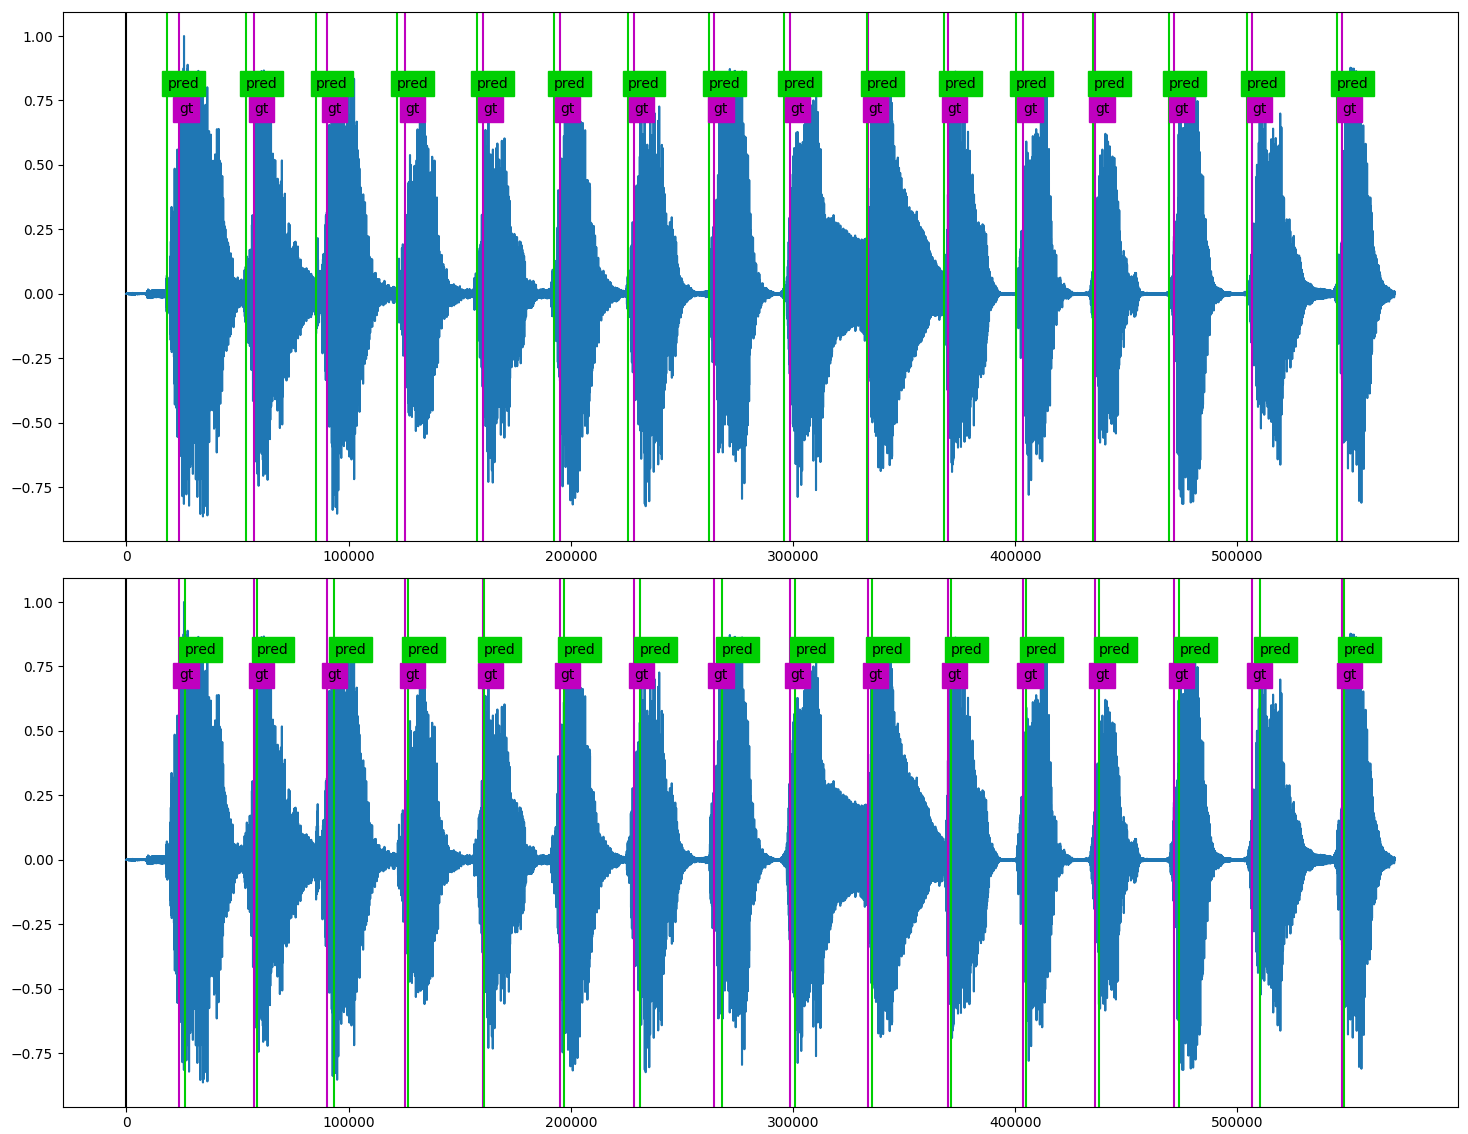
\includegraphics[width=\columnwidth]{discussion/hodmcod215.png}
    \caption{Predictions of Harmonic Onset Detector (top) and MC-OnsetDetector on a strummed chords. The algorithms aim at different locations of the chords. Due to long duration of the strums, some of the predictions are not accepted. F-scores are 0.44 and 0.55. (Purple lines: ground truth onsets, Green lines: onset predictions)}
    \label{fig:hodmcod215}
\end{figure}

\newpage


